\documentclass[12pt,a4paper]{article}
\usepackage{../../../../vkCourseML}
\title{Машинное обучение, ФКН ВШЭ\\Семинар №23}
\begin{document}
\author{}
\date{}
\maketitle

\section{Обучение модели попарных соотношений}

Ранее в курсе мы рассматривали задачи обучения с учителем, в которых данные имеют  вид $\{(x_i, y_i)\}_{i=1}^\ell$, где $x_i$ "--- вектор признаков, а $y_i$ "--- таргет, который необходимо предсказать по признакам (задачи классификации и регрессии). Также мы рассматривали задачи, где данные имеют вид $\{x_i\}_{i=1}^\ell$ – задачи кластеризации или задачи понижения размерности. 
\par На лекции мы рассмотрели новую постановку — задачу ранжирования и кратко рассмотрели существующие подходы (pointwise, pairwise, listwise). Несмотря на то, что во всех подходах целью является верное ранжирование объектов, считается, что заранее известно некоторое истинное значение релевантности (которое может быть основано на некоторой оценке ассессора, клике по документу или каком-либо другом сигнале), которое используется в оптимизируемом функционале качества. Однако зачастую данные в подобных задачах представлены лишь попарными взаимодействиями между объектами, то есть для некоторого набора объектов $\{x_i\}_{i=1}^n$ обучающая выборка представлена случайным подмножеством попарных соотношений: $\{ x_{i_k} > x_{j_k} \}_{k=1}^\ell$. Также для таких соотношений может быть известен некий контекст.
\par Далее мы будем рассматривать модели для попарных соотношений в контексте матчей между двумя игроками $x_i, \, x_j$, при этом наши рассуждения могут быть полностью перенесены на все остальные случаи применения этих моделей.

В общем случае данные о попарных соотношениях выглядят следующим образом: 
\begin{itemize}
	\item признаки объектов "--- для каждого игрока известно его признаковое описание $x_i \in \mathbb{R}^d$ (id, вес, рост, национальность и т.п.);
	\item признаки контекста "--- для каждого матча известно его признаковое описание $z_k \in \mathbb{R}^{D}$ (погода, время, место и т.п.);
	\item набор соотношений "--- история матчей в виде троек $\{ (x_{i_k}, x_{j_k}, z_k)\}$, где на первом месте стоит победитель матча.
\end{itemize} 
\newpage

\begin{vkProblem}
	Придумайте признаки объектов и признаки контекста для следующих задач:
	\begin{itemize}
		\item игра в теннис,
		\item рекомендации ресторанов,
		\item идентификация личности,
		\item клики на поисковую выдачу.
	\end{itemize}
\end{vkProblem}
\begin{esSolution}
	\begin{itemize}
		\item \textbf{В игре в теннис} объектом является игрок (теннисист), а соотношением является матч между двумя игроками. Таким образом, признаками игрока могут быть: пол, возраст, национальность, рост, вес и т.д. Признаками контекста матча могут быть: тип покрытия корта, погодные условия во время матча, уровень турнира, в рамках которого состоялась встреча.
		\item \textbf{При рекомендации ресторанов} объектом является ресторан, а соотношением является событие, когда пользователь предпочёл один ресторан другому. Признаками ресторана могут быть: тип кухни, средний чек, месторасположение, наличие детской комнаты, оценка пользователей. В качестве признаков контекста можно использовать признаки пользователя, который выбирал между ресторанами: где он выбирал ресторан (сайт или мобильное приложение), как составил запрос, в какое время он выбирал рестораны.
		\item \textbf{Для идентификации личности} можно поставить следующую задачу – есть входная фотография человека, фотография из базы данных, запись в базе данных, необходимо определить относится ли запись в базе данных и фотография из базы данных к человеку на входной фотографии. В качестве объекта мы выбираем фотографию человека, а в качестве контекста запись в базе данных. Признаковое описание фотографии можно получить, например, с помощью нейронных сетей, а признаковое описание объекта можно составить из записи в базе данных.
		\item Пусть у нас есть задача попарного сравнения документов в контексте одного запроса. Выборку набираем следующим образом – документ, на который кликнул человек в поисковой выдаче лучше всех документов, которые стоят выше него и на которые человек не кликнул. Признаки объекта это признаки документа: bm25, ctr, порядковый номер в выдаче и т.д., признаки контекста – длина запроса, размер выдачи на странице, версия поисковика (мобильная, браузерная) и т.д.
	\end{itemize}
\end{esSolution}

\subsection{Rote learning (зазубривание)}

Самая простая модель, которую можно обучить на этих данных это запоминание матрицы вероятностей для каждой пары игроков $(a,b)$. Искомую вероятность вычисляем по следующей формуле:

\begin{equation}
	P(x_i \text{ победит } x_j) = \frac{\sum_{k=1}^\ell [x_{i_k} = x_i][x_{j_k} = x_j]}{\sum_{k=1}^\ell ([x_{i_k} = x_i][x_{j_k} = x_j] + [x_{i_k} = x_j][x_{j_k} = x_i])}.
	\label{rote_prob}
\end{equation}

\par Так как могут быть ситуации, когда игроки никогда не встречались до этого (то есть в числителе и знаменателе стоят нули), то необходимо произвести сглаживание формулы \eqref{rote_prob}:

\begin{equation*}
	P(x_i \text{ победит } x_j) = \frac{\sum_{k=1}^\ell [x_{i_k} = x_i][x_{j_k} = x_j] + 1}{\sum_{k=1}^\ell ([x_{i_k} = x_i][x_{j_k} = x_j] + [x_{i_k} = x_j][x_{j_k} = x_i]) + 2}.
\end{equation*}

\textbf{Минусы}:
\begin{itemize}
	\item Необходимо очень много данных.
	\item Не учитывает никаких признаков.
	\item Не даёт оценки на исход матча между игроками, которые не встречались прежде.
\end{itemize}

\subsection{Модель Брэдли-Терри}

Следующая модель, которую мы рассмотрим, сопоставляет каждому игроку $x_i$ некоторый параметр $\gamma_i$, который может быть интерпретирован как сила (уровень) игрока. Вероятность победы игрока $x_i$ над игроком $x_j$, в такой модели записывается как:

\begin{align*}
	P(x_i \text{ победит } x_j) = \frac{\exp(\gamma_i)}{\exp(\gamma_i) + \exp(\gamma_j)}\\
	= \frac{1}{1 + \exp(\gamma_j - \gamma_i)} = \sigma(M(x_i, x_j)),
\end{align*}

где $\sigma(x)$ – сигма-функция, а функция $M(x_i,x_j) = \gamma_i - \gamma_j$ – функция матча~(matchup function). Функцию матча $M(x_i, x_j)$ можно задать произвольным образом, но при этом должны выполняться условия:

\begin{enumerate}
	\item $M(x_i, x_j) \in \mathbb{R}$, при этом положительные значения означают, что с большей вероятностью победит $i$, а отрицательные "--- наоборот. Вероятность победы любого из игроков при $M(x_i, x_j) = 0$ равняется $0.5$;
	\item при $M(x_i, x_j) \to +\infty$, $P(x_i \text{ победит } x_j) \to 1$, и наоборот;
	\item $M(x_i, x_j) = - M(x_j, x_i)$ "--- данное условие необходимо, чтобы выполнялось $P(x_i \text{ победит } x_j) = 1 - P(x_j \text{ победит } x_i)$.
\end{enumerate}

\textbf{Плюсы}:
\begin{itemize}
	\item Обладает небольшим числом параметров;
	\item Даёт оценки на исход матча между игроками, которые не встречались прежде.
\end{itemize}

\textbf{Минусы}:
\begin{itemize}
	\item По-прежнему не учитывает никаких признаков.
\end{itemize}

\begin{vkProblem}
	Запишите оптимизационную задачу, которую необходимо решить для настройки параметров этой модели. Рассчитайте градиенты полученного функционала.
\end{vkProblem}
\begin{esSolution}
	\begin{equation*}
		\sum_{k=1}^\ell \log P(x_{i_k} \text{ победит } x_{j_k}) \to \max_{\{\gamma_i\}}
	\end{equation*}
	
	\begin{align*}
		\frac{\partial}{\partial \gamma_s} \sum_{k=1}^\ell \log P(x_{i_k} \text{ победит } x_{j_k}) = & \frac{\partial}{\partial \gamma_s} \sum_{k=1}^\ell [i_k = s]\log P(x_{i_k} \text{ победит } x_{j_k})\\ 
		& + \frac{\partial}{\partial \gamma_s} \sum_{k=1}^\ell [j_k = s]\log P(x_{i_k} \text{ победит } x_{j_k})\\
		= \sum_{k=1}^\ell [i_k=s] &\bigg(\frac{1}{\sigma(M(s, x_{j_k}))} \sigma(M(s, x_{j_k})) ( 1 - \sigma(M(s, x_{j_k}))) \bigg)\\
		+ \sum_{k=1}^\ell -[j_k =s] &\bigg(\frac{1}{\sigma(M(x_{i_k}, s))} \sigma(M(x_{i_k}, s)) ( 1 - \sigma(M(x_{i_k}, s)))\bigg)\\
		= \sum_{k=1}^\ell [i_k=s] \bigg( &\frac{\exp(\gamma_{j_k})}{\exp(\gamma_s) + \exp(\gamma_{j_k})} \bigg) - \sum_{k=1}^\ell [i_k=s] \bigg( \frac{\exp(\gamma_s)}{\exp(\gamma_{i_k}) + \exp(\gamma_s)} \bigg)
	\end{align*}
\end{esSolution}

\subsection{Pairwise logistic regression model}

Модель Брэдли-Терри может быть легко расширена для учёта признаков игроков, если в качестве параметров рассматривать не $\gamma_i$, а обучить линейную модель для оценки силы игрока, то есть сила $\gamma_i$ игрока $x_i$ будет выражаться следующим образом:

\begin{equation*}
	\gamma_i = w^T x_i.
\end{equation*}

Заметим, что если в качестве признакового описания игрока мы возьмём его id, представленный с помощью one-hot-encode вектора, то получим модель Бредли-Терри в явном виде.

При обучении этой модели можно добавлять регуляризацию на веса $w$.

Тем не менее, модель по-прежнему не может учесть признаки матча. Действительно, попробуем добавить признаки матча $z_g$ к признаковому вектору каждого игрока:

\begin{equation*}
	M(a,b) = w^T\bigg(
	\begin{bmatrix}
	x_i\\
	z_k
	\end{bmatrix}
	-
	\begin{bmatrix}
	x_j\\
	z_k
	\end{bmatrix}
	 \bigg)
	= 
	w^T
	\begin{bmatrix}
	x_i - x_j\\
	0
	\end{bmatrix}.
\end{equation*}

Видим, что признаковое описание матча не влияет на функцию $M(x_i, x_j)$, а потому не участвует в оптимизируемом функционале. Попробуем переписать функцию $M(x_i, x_j)$ так, чтобы она явно учитывала признаки матча линейным образом: 
$$M(x_i, x_j) = w^T(x_i - x_j) + w_k^T z_k,$$
но заметим, что в этом случае не выполняется условие 3 для функции матча~$M(x_i, x_j)$.

\subsection{Blade-chest model}

Следующий подход, который мы рассмотрим, предлагает оригинальный вариант функции $M(a,b)$. Идея подхода заключается в том, что представление силы игрока одним числом плохо описывает данные, в частности, такая модель не может описать соотношение "камень-ножницы-бумага" между тремя игроками. Поэтому предлагается обучать для каждого игрока $x_i$ два вектора "--- $x_i^{\text{blade}}$~и~$x_i^{\text{chest}}$. Чтобы оценить вероятность победы игрока $x_i$ над игроком $x_j$ необходимо сравнить расстояния между представлениями "--- если $x_i^{\text{blade}}$ ближе к $x_j^{\text{chest}}$, чем $x_j^{\text{blade}}$ ближе к $x_i^{\text{chest}}$, то вероятнее победит игрок $x_i$. Названия представлений (клинок и грудь) дают понятную интерпретацию этих векторов. На рис. \ref{blade-chest} эта интерпретация проиллюстрирована.

\begin{figure}[h!]
\centering
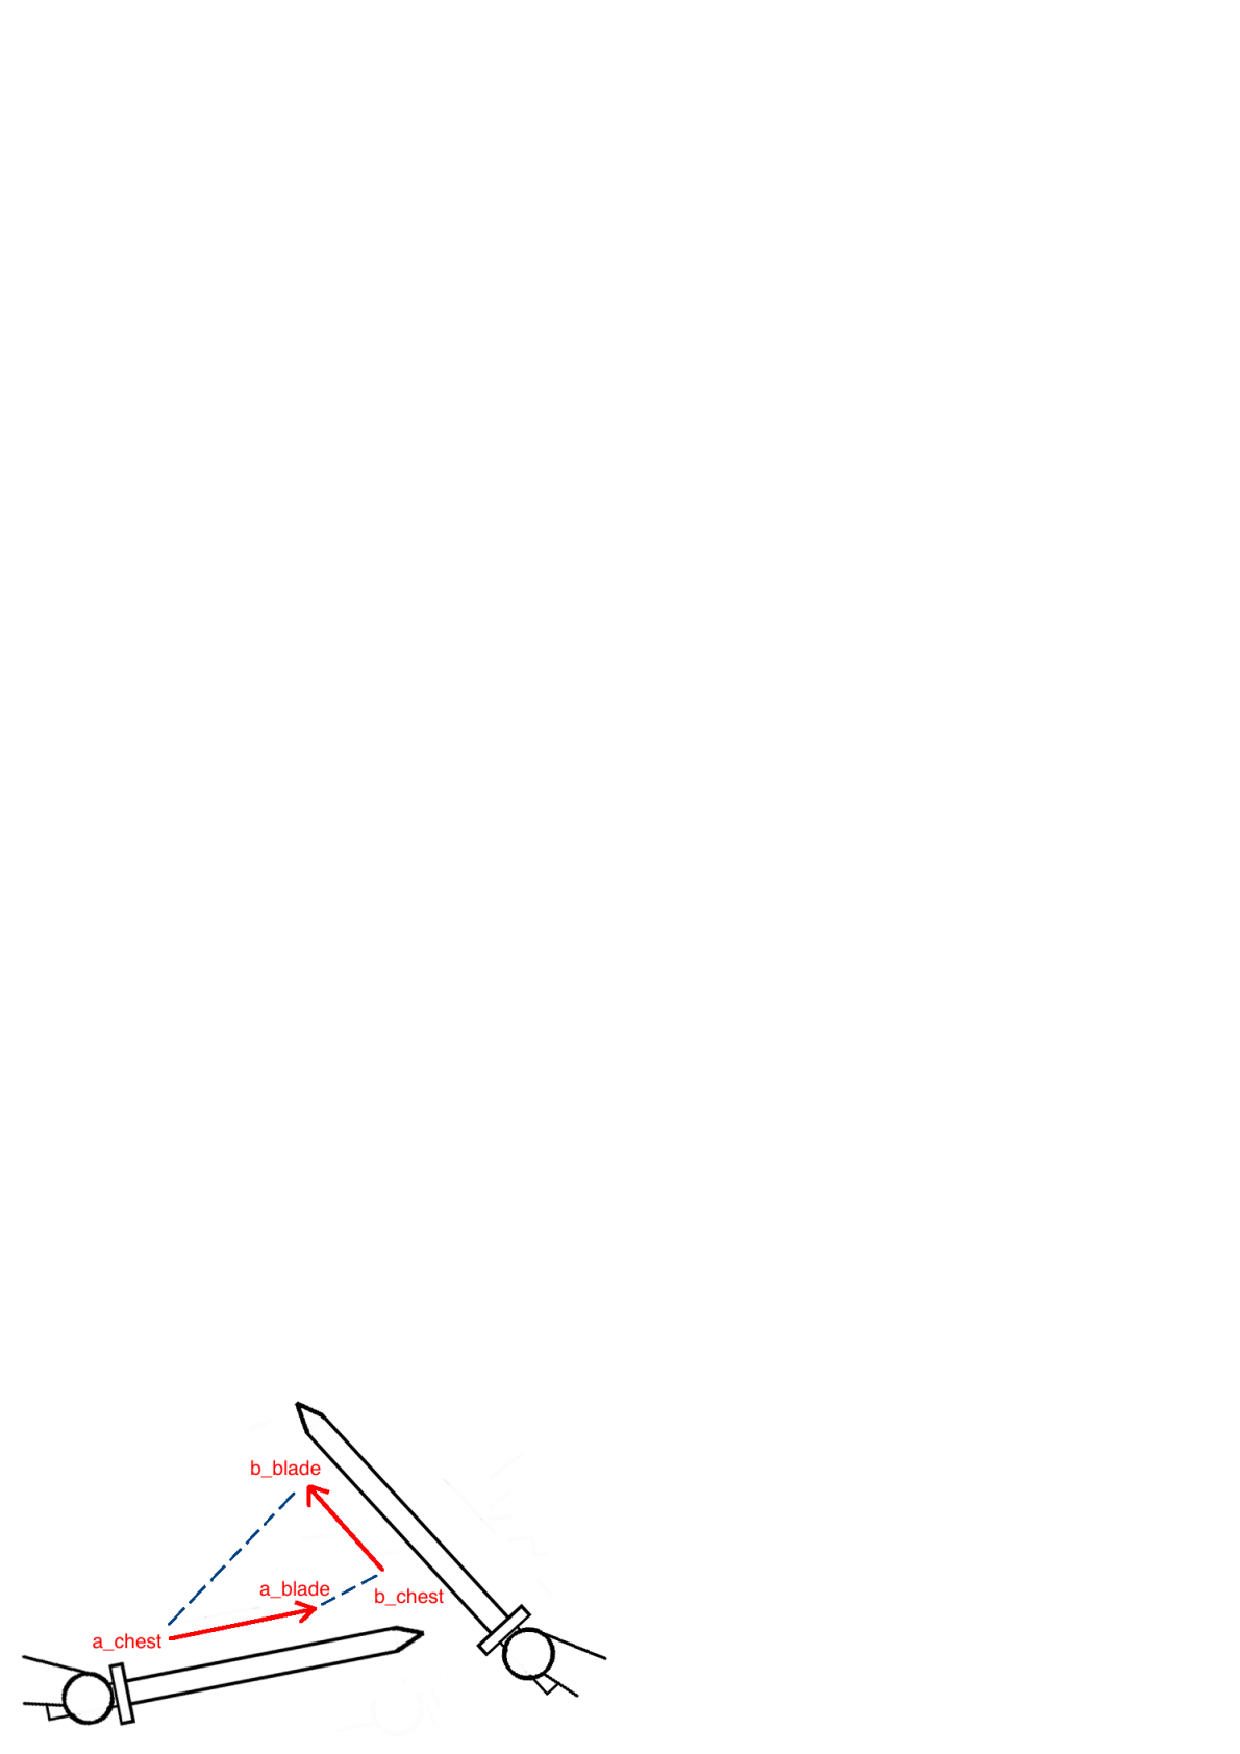
\includegraphics[scale=0.8]{blade-chest.png}
\caption{На рисунке проиллюстрирована интерпретация обучаемых представлений. Между игроками $a$ и $b$ происходит поединок. Видно, что клинок игрока $a$ ближе к груди игрока $b$, чем клинок игрока $b$ к груди игрока $a$, следовательно игрок $a$ имеет более высокие шансы на победу.}
\label{blade-chest}
\end{figure}

Функция $M(x_i,x_j)$ в этой модели записывается как
\begin{equation*}
	M(x_i, x_j) = \Vert x_j^{\text{blade}} - x_i^{\text{chest}} \Vert^2 - \Vert x_i^{\text{blade}} - x_j^{\text{chest}} \Vert^2.
\end{equation*}
\newpage

Также можно записать функцию $M(x_i,x_j)$ альтернативным способом, используя скалярное произведение:

\begin{equation*}
	M(x_i, x_j) = \langle x_i^{\text{blade}}, x_j^{\text{chest}} \rangle - \langle x_j^{\text{blade}}, x_i^{\text{chest}} \rangle.
\end{equation*}

В предыдущей модели мы использовали линейную комбинацию признаков для оценки силы игрока. Тот же подход мы можем использовать для оценки искомых представлений. Кроме того, помимо линейной комбинации признаков игроков, можно также использовать любую дифференцируемую функцию для оценки этих векторов. В общем виде можем записать:
\begin{align*}
	x_i^{\text{blade}} = f_{\text{blade}}(B x_i)\\
	x_j^{\text{blade}} = f_{\text{blade}}(B x_j)\\
	x_i^{\text{chest}} = f_{\text{chest}}(C x_i)\\
	x_j^{\text{chest}} = f_{\text{chest}}(C x_j).
\end{align*}

Получение данных представлений можно рассматривать как полносвязный слой нейросети с нелинейностью. Без ограничений общности мы можем использовать любые архитектуры нейросетей для обучения данных представлений.

В данной модели мы можем учесть признаки игры $z_k$ одним из двух способов:
\begin{enumerate}
	\item Первый способ заключается в добавлении признаков игры к признаковому описанию каждого игрока:
	
	\begin{align*}
		x_i^{\text{blade}} = & f_{\text{blade}}\bigg(B \begin{bmatrix} x_i\\ z_k \end{bmatrix}\bigg),\\
		x_i^{\text{chest}} = & f_{\text{chest}}\bigg(C \begin{bmatrix} x_i\\ z_k \end{bmatrix}\bigg).
	\end{align*}
	\item Второй способ заключается в \textbf{поэлементном} домножении векторов представлений на векторы представлений матча, полученные из признакового описания матча аналогично векторам $x^{\text{blade}}, \, x^{\text{chest}}$, то есть:
	
	\begin{align*}
		x_i^{\text{blade}} = f_{\text{blade}}(B x_i) \cdot f_{\text{match}}(B^\prime z_k),\\
		x_i^{\text{chest}} = f_{\text{chest}}(C x_i) \cdot f_{\text{match}}(C^\prime z_k).
	\end{align*}
	
\end{enumerate}


\end{document}
